\chapter{Planificación y cronograma}\label{ch:anexo5}
El control de horas del proyecto puede verse representado en la figura \ref{fig:figuraCrono}, donde están indicadas las horas dedicadas a cada tarea del proyecto cada semana de la duración del mismo. Cabe aclarar que no se ha llevado control de horas de la tarea
``investigación y lectura de documentación'' ya que ha sido una tarea presente durante toda la duración del proyecto.
\begin{figure}[H]
  \centering
  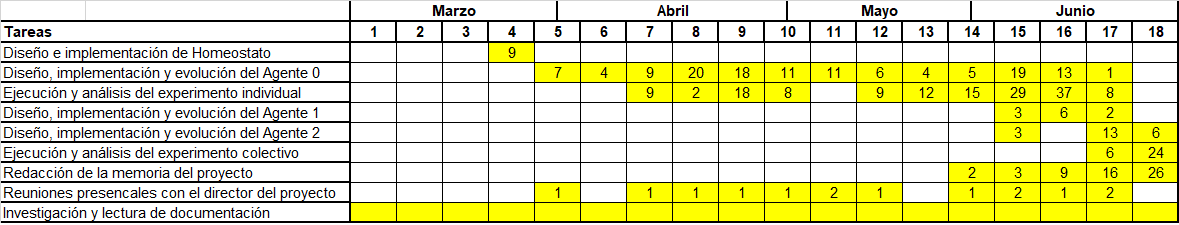
\includegraphics[width=1.0\textwidth]{Imagenes/Cronograma}
	\caption{Cronograma del proyecto dividido por semanas, incluyendo las horas dedicadas cada semana a cada tarea.}
	\label{fig:figuraCrono}
\end{figure}

En total se han invertido 417 horas a la realización de este Trabajo de Fin de Grado.
